\documentclass[10pt,a4paper]{article}
\usepackage[margin=2.0cm]{geometry}
\usepackage[T1]{fontenc}
\usepackage{lmodern}
\usepackage{microtype}
\usepackage[table]{xcolor}
\usepackage{booktabs,array}
\usepackage{tabularx}
\usepackage{amsmath,amssymb}
\usepackage{graphicx}
\usepackage{tikz}
\usetikzlibrary{arrows.meta,positioning,calc}
\usepackage{float}
\usepackage{placeins}
\usepackage{xr-hyper}
\usepackage[hidelinks]{hyperref}
\externaldocument[supp-]{contextual_sparse_etm_supplement}[contextual_sparse_etm_supplement.pdf]
\usepackage{enumitem}
\usepackage{fancyhdr}
\definecolor{accent}{HTML}{1D4ED8}
\definecolor{accentlight}{HTML}{DBEAFE}
\definecolor{softgray}{HTML}{F3F4F6}
\definecolor{lossgold}{HTML}{C6922F}
\hypersetup{colorlinks=true,linkcolor=accent,urlcolor=accent,citecolor=accent,
pdftitle={Discovering Molecular Substructures from Mass Spectra with Neural Topic Models}}
% Current-model numbers come only from the selected whole-spectrum model.
% Generated: chosen full-document model; validation only.
\newcommand{\CurrentEvaluableMean}{665.7}
\newcommand{\CurrentEvaluableSD}{7.6}
\newcommand{\CurrentUsefulMean}{390.7}
\newcommand{\CurrentUsefulSD}{2.1}
\newcommand{\CurrentSOSMean}{0.629}
\newcommand{\CurrentSOSSD}{0.002}
\newcommand{\CurrentNLLMean}{9.525}
\newcommand{\CurrentNLLSD}{0.023}
\newcommand{\CurrentEffectiveMean}{3.72}
\newcommand{\CurrentEffectiveSD}{0.03}
\newcommand{\CurrentWinnersMean}{807.3}
\newcommand{\CurrentWinnersSD}{9.1}
\newcommand{\ReferenceLDAEvaluable}{578.0}
\newcommand{\ReferenceLDAEvaluableSD}{5.0}
\newcommand{\ReferenceLDAUseful}{351.7}
\newcommand{\ReferenceLDAUsefulSD}{7.0}
\newcommand{\ReferenceLDASOS}{0.639}
\newcommand{\ReferenceLDASOSSD}{0.003}
\newcommand{\ReferenceLDANLL}{9.693}
\newcommand{\ReferenceLDANLLSD}{0.004}
\newcommand{\ReferenceLDAEffective}{9.26}
\newcommand{\ReferenceLDAEffectiveSD}{0.09}
\newcommand{\ReferenceCanonicalEvaluable}{202.7}
\newcommand{\ReferenceCanonicalEvaluableSD}{5.5}
\newcommand{\ReferenceCanonicalUseful}{125.0}
\newcommand{\ReferenceCanonicalUsefulSD}{6.1}
\newcommand{\ReferenceCanonicalSOS}{0.637}
\newcommand{\ReferenceCanonicalSOSSD}{0.006}
\newcommand{\ReferenceCanonicalNLL}{8.707}
\newcommand{\ReferenceCanonicalNLLSD}{0.029}
\newcommand{\ReferenceCanonicalEffective}{40.75}
\newcommand{\ReferenceCanonicalEffectiveSD}{1.09}
\newcommand{\CurrentUsefulDifference}{+39.0}

\newcommand{\ChemPrimaryStrata}{158}
\newcommand{\ChemFixedCompounds}{64}
\newcommand{\ChemSelectedEligibleMin}{657}
\newcommand{\ChemSelectedEligibleMax}{671}
\newcommand{\ChemSelectedSupportedMin}{799}
\newcommand{\ChemSelectedSupportedMax}{817}
\newcommand{\ChemLDAEligibleMin}{573}
\newcommand{\ChemLDAEligibleMax}{583}
\newcommand{\ChemLDASupportedMin}{933}
\newcommand{\ChemLDASupportedMax}{959}
\newcommand{\ChemLDASingletonEligible}{75.3}
\newcommand{\ChemLDARecurring}{502.7}
\newcommand{\ChemLDARecurringSD}{13.0}
\newcommand{\ChemLDASingleton}{132.7}
\newcommand{\ChemLDASingletonSD}{12.9}
\newcommand{\ChemLDABackground}{0.604}
\newcommand{\ChemLDABackgroundSD}{0.002}
\newcommand{\ChemLDAExcess}{0.035}
\newcommand{\ChemLDAExcessSD}{0.001}
\newcommand{\ChemLDASOSTopics}{9.7}
\newcommand{\ChemLDASOSTopicsSD}{3.5}
\newcommand{\ChemLDAFeatureTopics}{12.0}
\newcommand{\ChemLDAFeatureTopicsSD}{3.0}
\newcommand{\ChemSelectedSingletonEligible}{151.0}
\newcommand{\ChemSelectedRecurring}{514.7}
\newcommand{\ChemSelectedRecurringSD}{14.2}
\newcommand{\ChemSelectedSingleton}{197.0}
\newcommand{\ChemSelectedSingletonSD}{8.9}
\newcommand{\ChemSelectedBackground}{0.594}
\newcommand{\ChemSelectedBackgroundSD}{0.003}
\newcommand{\ChemSelectedExcess}{0.035}
\newcommand{\ChemSelectedExcessSD}{0.003}
\newcommand{\ChemSelectedSOSTopics}{10.7}
\newcommand{\ChemSelectedSOSTopicsSD}{1.5}
\newcommand{\ChemSelectedFeatureTopics}{10.0}
\newcommand{\ChemSelectedFeatureTopicsSD}{1.7}
\newcommand{\ChemLDAScaffoldExcess}{0.029}
\newcommand{\ChemLDAScaffoldFeatureTopics}{3.0}
\newcommand{\ChemSelectedScaffoldExcess}{0.032}
\newcommand{\ChemSelectedScaffoldFeatureTopics}{3.0}
\newcommand{\ChemSelectedMatchMedian}{0.625}
\newcommand{\ChemSelectedReciprocal}{0.673}
\newcommand{\ChemSelectedCompoundMatch}{0.012}
\newcommand{\ChemSelectedRedundantMedian}{0.093}
\newcommand{\ChemSelectedRepeatedMAG}{96.3}
\newcommand{\ChemSelectedRepeatedMAGPercent}{11.9}
\newcommand{\ChemSelectedReferenceMedian}{0.201}
\newcommand{\ChemSelectedReferenceOverlap}{0.066}
\newcommand{\ChemSelectedReferenceAnyOverlap}{662.0}
\newcommand{\ChemLDAMatchMedian}{0.529}
\newcommand{\ChemLDAReciprocal}{0.666}
\newcommand{\ChemLDACompoundMatch}{0.000}
\newcommand{\ChemLDARedundantMedian}{0.025}
\newcommand{\ChemLDARepeatedMAG}{47.7}
\newcommand{\ChemLDARepeatedMAGPercent}{7.8}
\newcommand{\ChemLDAReferenceMedian}{0.188}
\newcommand{\ChemLDAReferenceOverlap}{0.069}
\newcommand{\ChemLDAReferenceAnyOverlap}{531.3}
\newcommand{\ChemCrossMatchMedian}{0.404}
\newcommand{\ChemRawReferences}{255}
\newcommand{\ChemUniqueReferences}{234}
\newcommand{\ChemScorableReferences}{234}
\newcommand{\ChemExcludedReferences}{0}
\newcommand{\ChemConflictingReferences}{8}

\newcommand{\OverlapNNChemicalDefined}{3,088}
\newcommand{\OverlapNNChemicalUndefined}{0}
\newcommand{\OverlapNNAllCos}{0.650}
\newcommand{\OverlapNNRecurringCos}{0.625}
\newcommand{\OverlapNNCompound}{0.171}
\newcommand{\OverlapNNChemical}{0.423}
\newcommand{\OverlapNNFragment}{0.718}
\newcommand{\OverlapNNLoss}{0.379}
\newcommand{\OverlapNNChannelCos}{0.508}
\newcommand{\OverlapNNNoMAGFilterCos}{0.635}
\newcommand{\OverlapNLChemicalDefined}{4,631}
\newcommand{\OverlapNLChemicalUndefined}{1}
\newcommand{\OverlapNLAllCos}{0.454}
\newcommand{\OverlapNLRecurringCos}{0.420}
\newcommand{\OverlapNLCompound}{0.075}
\newcommand{\OverlapNLChemical}{0.260}
\newcommand{\OverlapNLFragment}{0.550}
\newcommand{\OverlapNLLoss}{0.006}
\newcommand{\OverlapNLChannelCos}{0.339}
\newcommand{\OverlapNLNoMAGFilterCos}{0.516}
\newcommand{\OverlapLNChemicalDefined}{4,521}
\newcommand{\OverlapLNChemicalUndefined}{3}
\newcommand{\OverlapLNAllCos}{0.454}
\newcommand{\OverlapLNRecurringCos}{0.460}
\newcommand{\OverlapLNCompound}{0.089}
\newcommand{\OverlapLNChemical}{0.307}
\newcommand{\OverlapLNFragment}{0.547}
\newcommand{\OverlapLNLoss}{0.007}
\newcommand{\OverlapLNChannelCos}{0.337}
\newcommand{\OverlapLNNoMAGFilterCos}{0.403}
\newcommand{\OverlapLLChemicalDefined}{3,011}
\newcommand{\OverlapLLChemicalUndefined}{5}
\newcommand{\OverlapLLAllCos}{0.547}
\newcommand{\OverlapLLRecurringCos}{0.525}
\newcommand{\OverlapLLCompound}{0.167}
\newcommand{\OverlapLLChemical}{0.382}
\newcommand{\OverlapLLFragment}{0.705}
\newcommand{\OverlapLLLoss}{0.003}
\newcommand{\OverlapLLChannelCos}{0.394}
\newcommand{\OverlapLLNoMAGFilterCos}{0.524}
\newcommand{\OverlapMedianCos}{0.422}
\newcommand{\OverlapMedianSecondCos}{0.107}
\newcommand{\OverlapMedianFragmentShared}{1}
\newcommand{\OverlapMedianLossShared}{0}
\newcommand{\OverlapUpperCos}{0.887}
\newcommand{\OverlapUpperSecondCos}{0.087}
\newcommand{\OverlapUpperFragmentShared}{2}
\newcommand{\OverlapUpperLossShared}{0}
\newcommand{\OverlapMultipleCos}{0.522}
\newcommand{\OverlapMultipleSecondCos}{0.324}
\newcommand{\OverlapMultipleFragmentShared}{5}
\newcommand{\OverlapMultipleLossShared}{0}
\newcommand{\OverlapMultipleSecondFragmentShared}{3}
\newcommand{\OverlapMultipleSecondLossShared}{0}

\pagestyle{fancy}
\fancyhf{}
\setlength{\headheight}{14pt}
\setlength{\headsep}{18pt}
\cfoot{\thepage}
\renewcommand{\headrulewidth}{0pt}
\fancypagestyle{plain}{\fancyhf{}\cfoot{\thepage}\renewcommand{\headrulewidth}{0pt}}
\setlist{nosep,leftmargin=*}
\newcommand{\softmax}{\operatorname{softmax}}
\newcommand{\normalize}{\operatorname{normalize}}
\newcommand{\entmax}{\operatorname{entmax}_{1.5}}
\newcommand{\KL}{\operatorname{KL}}
\newcommand{\ctxscale}{\lambda_{\mathrm{ctx}}}
\tikzset{
  modelnode/.style={draw=black!55,rounded corners=2pt,align=center,
    minimum height=1.05cm,inner sep=3pt,font=\footnotesize,text width=2.35cm},
  dataflow/.style={-{Latex[length=2mm]},line width=0.55pt,draw=black!70},
  pipelinebox/.style={draw=black!55,fill=softgray,rounded corners=2pt,
    align=center,minimum height=1.2cm,text width=2.5cm,inner sep=3pt,font=\scriptsize}
}
\title{Discovering Molecular Substructures from Mass Spectra\\with Neural Topic Models}
\author{}
\date{}
\begin{document}
\maketitle

\begin{abstract}
Substructure discovery from mass spectra seeks recurring fragmentation
patterns and an interpretable account of how they combine within individual
spectra. We present Contextual Sparse ETM, an adaptation of the published
Embedded Topic Model that retains its embedding-based decoder and Gaussian
inference network. Three enhancements balance fragment and neutral-loss
probabilities, use whole-spectrum evidence to guide inference, and allow
exactly zero topic weights through 1.5-entmax.
Across three training runs evaluated on 3,889 MS$^{n}$Lib validation spectra, the selected model
produces \CurrentUsefulMean{}$\pm$\CurrentUsefulSD{} motifs meeting the
specified chemical screening criterion, compared with
\ReferenceLDAUseful{}$\pm$\ReferenceLDAUsefulSD{} for Tomotopy LDA.
Completion negative log-likelihood is lower, but mean chemical overlap among
evaluable motifs is also lower. The median entropy-effective number of topics
per spectrum is \CurrentEffectiveMean{}$\pm$\CurrentEffectiveSD{}.
Matched-background analysis finds similar small excess chemical overlap in
both models, and much of the additional evaluable neural inventory has
single-compound support. Cross-model matching identifies shared spectral
patterns, with stronger agreement in fragments than losses and limited
agreement in supporting compounds. These findings support a broader candidate
inventory with compact per-spectrum explanations, rather than more confirmed
substructures. Because the validation data also informed model selection,
independent evaluation and structural follow-up remain necessary.
\end{abstract}

\section{Introduction}

Untargeted metabolomics uses mass spectrometry to survey small molecules
without restricting an experiment to a predefined list of compounds.
Tandem mass spectrometry (MS/MS) adds structural information by fragmenting
an isolated precursor ion and recording the mass-to-charge ratios ($m/z$)
and intensities of the resulting ions. Relating those patterns to molecular
structures remains difficult: different molecules can share fragments, and
the spectrum of one molecule can change with acquisition conditions.
Reference-library matching is valuable when suitable standards are available,
but incomplete library coverage motivates complementary ways to interpret
unidentified spectra \cite{huber2021,vanderhooft2016}.

Substructure discovery asks a different question from complete molecular
identification. Instead of selecting one molecule for each spectrum, it seeks
recurring evidence for chemical building blocks across many spectra.
MS2LDA casts this as topic modeling: spectra are documents, binned fragments
and neutral losses are words, and recurring word distributions are
\emph{Mass2Motifs} \cite{vanderhooft2016}. A spectrum can contain several
motifs, and a motif can occur in chemically different molecules. This is useful
for relating compounds whose complete spectra need not be close matches.
Each pattern suggests a possible chemical interpretation, but does not by
itself identify a unique substructure or establish a fragmentation pathway.

MS2LDA 2.0 makes this workflow substantially more practical through the
Tomotopy topic-modeling backend, improved software interfaces and automated
Mass2Motif Annotation Guidance (MAG) \cite{torresortega2026}. These advances
address computational and annotation bottlenecks; they do not make every
learned topic chemically informative. Its library benchmark includes motifs
that cannot be retained after annotation refinement, lack associated molecules,
or have weak structural agreement. We therefore focus on improving the learned
motifs and their assignments to spectra, while retaining these software and
annotation advances.

The existing LDA model learns a topic--word probability table and already uses
both fragment/loss co-occurrence and mixtures of topics within a spectrum.
It does not explicitly share statistical strength through continuous
spectral-word embeddings or learn a reusable neural inference function.
LDA can nevertheless represent both concentrated mixtures and contextual
dependence. We investigate whether an embedding-based neural alternative
can increase the number of motifs meeting our chemical screening criterion
while maintaining compact per-spectrum mixtures. We do not attempt automatic
selection of the number of topics, removal of reference-library bias, or
tokenization-free spectral modeling.

We build on the published Embedded Topic Model (ETM) \cite{dieng2020}.
ETM represents each topic by a vector in the same space as the spectral-word
embeddings. The topic--word inner products define a distribution over words;
a multilayer perceptron (MLP) infers how topics combine within each spectrum.
We adapt this model in three ways:
\begin{enumerate}
 \item \emph{Balanced fragment and loss emissions.} Give the two spectral
 channels equal probability mass within each topic, so they do not compete
 for the topic's total mass.
 \item \emph{Whole-spectrum contextual evidence.} Match a word together with
 its surrounding spectrum to the topic embeddings, and use the pooled
 evidence to correct the encoder's Gaussian mean.
 \item \emph{Sparse topic mixtures.} Replace softmax with 1.5-entmax, allowing
 weakly supported topics to receive exactly zero weight.
\end{enumerate}
Figure~\ref{fig:enhancements} gives a worked illustration of each change.
The model retains ETM's shared topics, Gaussian latent representation and
variational training framework.

We evaluate the model in two settings: controlled synthetic spectra, where
the planted motifs are known, and real reference spectra, where Tomotopy LDA
is the primary comparator. Plain ETM provides a secondary baseline for
assessing the combined enhancements. Our contribution is a spectral adaptation
of an established neural topic model, evaluated for both motif recovery and
practical substructure discovery.

\section{Related work}

\paragraph{Spectral topics and reusable motif annotations.}
LDA represents documents as mixtures of latent topics, with a probability
distribution over words for each topic \cite{blei2003}. The original MS2LDA
transfers that construction to fragments and neutral losses, enabling
unsupervised discovery of patterns shared across spectra \cite{vanderhooft2016}.
Subsequent work introduced MotifDB to store, share and reuse annotated
Mass2Motifs, linking discovery with community annotation
\cite{rogers2019}. MS2LDA 2.0 extends the practical workflow with scalable
fitting and MAG \cite{torresortega2026}. We retain its motif interpretation
and annotation framework so that the main comparison concerns the topic model,
not replacement of the entire discovery pipeline.

\paragraph{Learning relationships between spectral features.}
Skip-gram with negative sampling learns word coordinates from co-occurrence
\cite{mikolov2013}. Spec2Vec applies this idea to mass spectra: fragments
and losses receive embeddings that support spectrum-level similarity
\cite{huber2021}. This motivates using learned spectral relationships rather
than treating every vocabulary entry as unrelated, although an embedding
distance is not itself proof of a shared substructure. Our ETM uses word
embeddings trained only on its training spectra. The pretrained Spec2Vec
model used by MAG is a separate annotation asset, not the ETM representation.
More recently, DreaMS learns representations directly from large collections
of spectra through self-supervised training \cite{bushuiev2026}. Such models
could provide future spectrum encoders; they are not used in these experiments.

\paragraph{Neural probabilistic topic models.}
Autoencoding variational inference replaces repeated document-specific
optimization with a learned recognition network. The AVITM framework also
introduced ProdLDA, which changes the observation combination from LDA's
mixture to a product of experts \cite{srivastava2017}. ETM instead uses
embedding inner products to parameterize topic--word distributions while
retaining an additive topic mixture \cite{dieng2020}. This makes ETM a
particularly transparent base for Mass2Motifs: each topic still has a
normalized distribution over identifiable fragment/loss words. We therefore
retain ETM's Gaussian latent variables, two-hidden-layer MLP and variational
training objective. The official Pyro tutorial illustrates a ProdLDA
implementation \cite{pyroprodlda}; our experiments use neither that implementation
nor its product-of-experts decoder.

\paragraph{Contextual inference and sparse probability maps.}
Topic-aware neural inference predates this work. For example, TAN-NTM uses
topic attention over contextual sequence representations before variational
inference \cite{panwar2021}. Our permutation-invariant inference path combines
each word embedding with the mean embedding of the whole spectrum, compares
the resulting vector with the decoder's topic vectors, and adds the pooled
evidence to the Gaussian posterior mean.
There is no recurrent sequence encoder or second topic dictionary.
The entmax family provides published probability mappings that can produce
exact zeros \cite{peters2019}. We use its 1.5 form to modify ETM's topic
mixtures. Both attention and sparse probability maps are established methods;
here we combine them within ETM to model spectral motifs.

\section{Materials and methods}

We first describe the spectral input and base ETM, then explain the three
enhancements and how they fit together. The main text retains the model's
probabilistic structure and worked examples. Full notation, mathematical
details and reproducible protocols are in the accompanying
\href{contextual_sparse_etm_supplement.pdf}{Supplementary Information}.

\subsection{Spectra, spectral words and evaluation data}

We use the positive-ion MS$^{n}$Lib benchmark distributed with MS2LDA 2.0
\cite{brungs2025,msnlibdata}. Filtering leaves 38,888 of 41,568 input spectra.
Each retained peak contributes a fragment word and, where applicable, a
precursor-minus-fragment neutral-loss word. Masses are rounded to two decimal
places; a peak with relative intensity $I$ contributes $\operatorname{round}(100I)$
copies of each word. These are intensity-derived pseudo-counts, rather than
independent ion counts. Figure~\ref{fig:data} gives a numerical example.
The model reconstructs the count vector $c_d$ for spectrum $d$, while the
encoder receives its normalized version $x_d=c_d/\sum_w c_{dw}$.

Molecules are grouped by connectivity and scaffold before splitting, giving
27,222 training, 3,889 validation and 7,777 reserved test spectra, with no
compound or split-group overlap. The vocabulary contains 21,233 words
occurring in at least three training spectra. We learn 48-dimensional word
embeddings from training spectra using skip-gram with negative sampling
\cite{mikolov2013} and hold them fixed during topic-model fitting.
Neither validation spectra nor chemical labels train the vocabulary,
embeddings or model weights. The reported results use development-validation
data that also informed model selection; the reserved test set is not used
for the comparisons reported here. It was examined during earlier development
and is therefore not an untouched confirmation set.
Filtering, tokenization and splitting details are in Supplementary
Section~\ref{supp-sec:data}.

% A numerical illustration of preprocessing, not an accepted one-peak spectrum.
% Coordinates are in centimetres at final size: do not shrink the text to fit.
\begin{figure}[H]
\centering
\begin{tikzpicture}[x=1cm,y=1cm,font=\fontsize{9}{11}\selectfont]
\path[use as bounding box] (0,0.2) rectangle (16.8,-7.4);
\node[anchor=west,font=\bfseries\fontsize{10}{12}\selectfont] at (0,0)
  {(a) One retained peak becomes two spectral words};

% The dashed precursor marker is a mass reference, not a measured intensity.
\node[anchor=west] at (0,-0.60) {Intensity};
\draw[black!65] (0.42,-2.80)--(4.0,-2.80);
\draw[black!65] (0.42,-2.80)--(0.42,-1.05);
\draw[black!65] (0.36,-1.05)--(0.48,-1.05);
\node[anchor=east] at (0.31,-1.05) {1};
\node[anchor=east] at (0.31,-2.80) {0};
\draw[accent,line width=1.6pt] (2.43,-2.80)--(2.43,-2.10);
\node[accent,anchor=south] at (2.43,-2.06) {0.40};
\draw[dashed,black!60,line width=0.6pt] (3.77,-2.80)--(3.77,-1.05);
\draw[black!65] (2.43,-2.80)--(2.43,-2.87);
\draw[black!65] (3.77,-2.80)--(3.77,-2.87);
\node[anchor=north] at (2.43,-2.91) {60.00};
\node[anchor=north] at (3.77,-2.91) {100.00};
\node[anchor=north] at (2.21,-3.27) {fragment};
\node[anchor=north] at (3.85,-3.27) {precursor};
\node[anchor=north west] at (0.42,-2.91) {$m/z$};
% A bracket, rather than an arrow, denotes the precursor-minus-fragment gap.
\draw[lossgold,line width=0.7pt]
  (2.43,-1.18)--(2.43,-0.94)--(3.77,-0.94)--(3.77,-1.18);
\node[lossgold!65!black,anchor=south] at (3.10,-0.90) {loss: 40.00};

\draw[dataflow] (4.38,-1.83)--(4.91,-1.83);
\node[anchor=west,font=\bfseries\fontsize{9}{11}\selectfont] at (5.13,-0.70)
  {Spectral word};
\node[anchor=east,font=\bfseries\fontsize{9}{11}\selectfont] at (9.55,-0.70)
  {Count};
\draw[black!35] (5.13,-0.98)--(9.55,-0.98);
\node[anchor=west,text=accent] at (5.13,-1.42) {\texttt{frag@60.0}};
\node[anchor=east] at (9.55,-1.42) {40};
\node[anchor=west,text=lossgold!65!black] at (5.13,-2.03) {\texttt{loss@40.0}};
\node[anchor=east] at (9.55,-2.03) {40};
\node[align=center] at (7.34,-2.84)
  {$\operatorname{round}(100\times0.40)=40$};
\node[align=center,text width=4.40cm] at (7.34,-3.32)
  {The two words keep one peak-group identity.};

\draw[dataflow] (9.79,-1.83)--(10.32,-1.83);
\node[align=center,font=\bfseries\fontsize{9}{11}\selectfont,text width=5.9cm]
  at (13.55,-0.70)
  {Accumulate over all retained peaks};
\node[align=center] at (13.55,-1.37) {Raw-count reconstruction target};
\node[align=center,font=\fontsize{11}{13}\selectfont] at (13.55,-1.83) {$c_d$};
\node[align=center] at (13.55,-2.49) {Normalized encoder input};
\node[align=center,font=\fontsize{11}{13}\selectfont] at (13.55,-3.02)
  {$x_d=c_d/N_d$};

\draw[black!20] (0,-3.88)--(16.8,-3.88);
\node[anchor=west,font=\bfseries\fontsize{10}{12}\selectfont] at (0,-4.22)
  {(b) Structure groups stay within one partition};
\node[anchor=west] at (0,-4.66)
  {38,888 filtered spectra; no shared compound or split group between partitions};

% Parallel roles, not a training-to-validation flow or a proportional bar chart.
\fill[accentlight] (0,-5.06) rectangle (5.28,-5.65);
\fill[softgray] (5.76,-5.06) rectangle (11.04,-5.65);
\fill[softgray] (11.52,-5.06) rectangle (16.8,-5.65);
\node[font=\bfseries\fontsize{9}{11}\selectfont] at (2.64,-5.35)
  {Training: 27,222};
\node[font=\bfseries\fontsize{9}{11}\selectfont] at (8.40,-5.35)
  {Validation: 3,889};
\node[font=\bfseries\fontsize{9}{11}\selectfont] at (14.16,-5.35)
  {Reserved test: 7,777};
\node[align=center,text width=5.0cm] at (2.64,-6.12)
  {Fit vocabulary, word vectors and model.};
\node[align=center,text width=5.0cm] at (8.40,-6.12)
  {Compare fitted models;\\results reported here.};
\node[align=center,text width=5.0cm] at (14.16,-6.12)
  {Excluded from these\\reported comparisons.};
\node[align=center] at (2.64,-6.65) {$V=21,233$; $E=48$};
\node[anchor=west,text width=16.8cm] at (0,-7.12)
  {Validation uses the vocabulary and word vectors fitted on training spectra.};
\end{tikzpicture}
\caption{Spectral representation and evaluation boundaries. (a) An illustrative
peak with normalized intensity 0.40 contributes paired fragment and neutral-loss
pseudo-counts when both words
occur in the training vocabulary. Accumulated raw counts train reconstruction;
normalized counts enter inference. The dashed precursor marker indicates mass,
not intensity. (b) Structure-grouped partitions have different roles; validation
does not fit the vocabulary or word embeddings.}
\label{fig:data}
\end{figure}


Controlled synthetic data provide a separate recovery experiment. Each
realization contains 18 planted motifs, one to three active motifs per
spectrum, and 800 training and 160 validation spectra. Shared anchors,
background peaks and intensity variation make recovery nontrivial. We fit
36 or 128 topics and assess recovery against the planted words and mixtures.
The generator and evaluation targets are described in Supplementary
Section~\ref{supp-sec:data}; they test statistical recovery, not a mechanism
of real molecular fragmentation.

\subsection{Base model: the published ETM}
\label{sec:base-etm}

ETM explains each spectrum as a mixture of shared topics. A topic is a
probability distribution over spectral words; its weight describes how
strongly it contributes to a spectrum. We use the published variant with
pre-fitted word embeddings \cite{dieng2020}. Let $\rho_w$ be the fixed vector
for word $w$, $\alpha_k$ the learned vector for topic $k$, $V$ the vocabulary
size, and $K$ the number of topics. The topic's word probabilities are
\begin{equation}
 \beta^{\mathrm{ETM}}_{kw}=
 \frac{\exp(\alpha_k^\top\rho_w)}
      {\sum_{v=1}^{V}\exp(\alpha_k^\top\rho_v)}.
 \label{eq:base-beta}
\end{equation}
The inner product measures topic--word compatibility. Words with similar
embeddings interact similarly with a topic vector, sharing information
across the vocabulary.

The generative model draws Gaussian topic scores $z_d$, converts them to
mixture weights $\theta_d$, and draws words from the weighted topic distributions:
\begin{equation}
 z_d\sim\mathcal N(0,I_K),\qquad
 \theta_d=\softmax(z_d),\qquad
 p(w\mid z_d)=\sum_{k=1}^{K}\theta_{dk}\beta^{\mathrm{ETM}}_{kw}.
 \label{eq:base-generator}
\end{equation}
For example, weights $(0.7,0.3)$ and a fragment with probabilities 0.4 and
0.1 under the two topics give predicted probability $0.7(0.4)+0.3(0.1)=0.31$.
The enhanced model retains this additive interpretation.

For an observed spectrum, the topic scores are unknown. A two-hidden-layer
MLP predicts a Gaussian mean $\mu_\phi(x_d)$ and log variance $\ell_\phi(x_d)$:
\begin{equation}
 q_\phi(z_d\mid x_d)=\mathcal N\!\left(\mu_\phi(x_d),
             \operatorname{diag}(\exp\ell_\phi(x_d))\right).
 \label{eq:base-posterior}
\end{equation}
The same encoder estimates the mixture for every spectrum, including a new
one. Training jointly fits topic vectors and encoder parameters, rewarding
reconstruction of observed counts while regularizing the inferred Gaussian
toward the standard-normal prior. This is ETM's variational training
framework. Supplementary Section~\ref{supp-sec:model} gives the full objective,
sampling calculation and notation.

\subsection{Enhancement 1: balance fragment and loss probabilities}

The first change is to the decoder. Fragments and losses give complementary
views of a peak, but base ETM puts all words into one softmax. A topic could
therefore assign 85\% of its probability to fragments and only 15\% to losses.
We normalize the words separately within each channel and give each channel
50\% of every topic's probability (Figure~\ref{fig:enhancements}a).
The model still learns which words matter within each channel.

% Schematic examples derived from the stated equations; not experiment data.
\begin{figure}[H]
\centering
\begin{minipage}[t]{0.32\textwidth}
\centering
\textbf{(a) Channel probability mass}\par\smallskip
\begin{tikzpicture}[x=1cm,y=1cm,font=\scriptsize]
\path[use as bounding box] (-0.1,-3.8) rectangle (5.1,0.4);
\node[anchor=west] at (0,0) {One softmax: illustrative topic};
\filldraw[fill=accent!70,draw=black!65] (0,-0.65) rectangle (3.74,-0.2);
\filldraw[fill=lossgold!70,draw=black!65] (3.74,-0.65) rectangle (4.4,-0.2);
\node at (1.87,-0.425) {fragments: 0.85};
\node at (4.07,-0.88) {losses: 0.15};
\draw[dataflow] (2.2,-1.05)--(2.2,-1.45);
\node[anchor=west] at (0,-1.8) {Separate normalizers};
\filldraw[fill=accent!70,draw=black!65] (0,-2.45) rectangle (2.2,-2.0);
\filldraw[fill=lossgold!70,draw=black!65] (2.2,-2.45) rectangle (4.4,-2.0);
\node at (1.1,-2.225) {fragments: 0.50};
\node at (3.3,-2.225) {losses: 0.50};
\node[align=left,text width=4.7cm,anchor=north west] at (0,-2.85)
{Topic probability mass is balanced.\\Observed counts are unchanged.};
\end{tikzpicture}
\end{minipage}\hfill
\begin{minipage}[t]{0.32\textwidth}
\centering
\textbf{(b) Whole-spectrum context}\par\smallskip
\begin{tikzpicture}[x=1cm,y=1cm,font=\scriptsize]
\path[use as bounding box] (-0.1,-3.8) rectangle (5.1,0.4);
\node[anchor=west] at (0,0) {Same word: $\widehat\rho_w=(1,0)$};
\draw[black!25] (0.35,-2.65)--(0.35,-0.45);
\draw[black!25] (0.1,-1.55)--(4.4,-1.55);
\draw[dataflow,draw=accent,line width=1pt]
  (0.35,-1.55)--(2.82,-0.727);
\draw[dataflow,draw=lossgold,line width=1pt]
  (0.35,-1.55)--(2.82,-2.373);
\draw[dataflow,line width=1pt] (0.35,-1.55)--(2.95,-1.55);
\node[anchor=west,text=accent] at (2.90,-0.70) {$h_{Aw}$};
\node[anchor=west] at (3.02,-1.55) {$\widehat\rho_w$};
\node[anchor=west,text=lossgold] at (2.90,-2.40) {$h_{Bw}$};
\node[align=left,text width=4.7cm,anchor=north west] at (0,-2.85)
{A: $s_A=(0.5,0.5)$\\B: $s_B=(0.5,-0.5)$\\
$h=\operatorname{normalize}(\widehat\rho_w+s)$};
\end{tikzpicture}
\end{minipage}\hfill
\begin{minipage}[t]{0.32\textwidth}
\centering
\textbf{(c) Sparse topic proportions}\par\smallskip
\begin{tikzpicture}[x=1cm,y=1cm,font=\scriptsize]
\path[use as bounding box] (-0.1,-3.8) rectangle (5.1,0.4);
\node[anchor=west] at (0,0) {Identical scores: $z=(1,0,-1)$};
\node[anchor=west] at (0,-0.4) {Softmax};
\filldraw[fill=accent!70,draw=black!65] (0,-1.05) rectangle (2.927,-0.65);
\filldraw[fill=lossgold!70,draw=black!65] (2.927,-1.05) rectangle (4.004,-0.65);
\filldraw[fill=black!20,draw=black!65] (4.004,-1.05) rectangle (4.4,-0.65);
\node[anchor=west] at (0,-1.3) {$(0.665,\;0.245,\;0.090)$};
\node[anchor=west] at (0,-1.8) {1.5-entmax};
\filldraw[fill=accent!70,draw=black!65] (0,-2.45) rectangle (3.655,-2.05);
\filldraw[fill=lossgold!70,draw=black!65] (3.655,-2.45) rectangle (4.4,-2.05);
\node[align=left,text width=4.7cm,anchor=north west] at (0,-2.85)
{$(0.831,\;0.169,\;0)$\\Topic 3 has exactly zero weight.};
\end{tikzpicture}
\end{minipage}
\caption{Illustrations of the three enhancements, not measured model outcomes.
In (a), bar length is total probability in each spectral channel. In (b),
a shared word vector is tilted by two different spectrum means, with context
strength one. The resulting unit directions are approximately
$h_{Aw}=(0.949,0.316)$ and $h_{Bw}=(0.949,-0.316)$; the axes are embedding
coordinates. In (c), colored segments are topic 1, topic 2 and
topic 3, in that order; each complete bar has unit mass.}
\label{fig:enhancements}
\end{figure}


The resulting $\beta$ remains a topic--word probability table and introduces
no additional learned parameter. Equal channel mass is a modeling assumption;
it does not force equal observed counts or equal gradient contributions.
The complete emission equation and its likelihood interpretation are in
Supplementary Section~\ref{supp-sec:balance}.

\subsection{Enhancement 2: use the surrounding spectrum to guide inference}

The second change is to the Gaussian mean inferred by the encoder. A fragment
can support different topics depending on which fragments and losses accompany
it. Although the base MLP already sees the full spectrum, we add an explicit
route that uses the decoder's embedding geometry to guide inference.

This route has four steps. We compute the intensity-weighted mean of the
spectrum's unit word vectors; add a learned multiple of that mean to each word
vector and normalize its direction; match that direction to its two closest
topic directions; then pool these matches with the observed word weights.
A centered log transformation converts the pooled evidence into a mean
correction $o_d$:
\begin{equation}
 m_d=\mu_\phi(x_d)+o_d.
 \label{eq:main-offset}
\end{equation}
The posterior remains Gaussian, with corrected mean $m_d$ and the MLP's
predicted variance. Uniform evidence gives zero correction. Top-2 matching
is a restriction per word, not a limit of two topics per spectrum. The
context pathway adds one learned strength scalar; it shares the decoder's
topic vectors.

Figure~\ref{fig:enhancements}b illustrates the idea. The same fragment vector
$(1,0)$, combined with spectrum means $(0.5,0.5)$ and $(0.5,-0.5)$ at context
strength one, points in different directions. Its stored vector is unchanged,
but its match to topics can differ. These illustrative coordinates explain
the calculation; they do not assign a chemical structure. The exact matching,
pooling and mean-correction formulas are in Supplementary
Section~\ref{supp-sec:context}.

\subsection{Enhancement 3: let weak topic weights become zero}

The third change maps Gaussian scores to sparse topic weights using
$\theta_d=\entmax(z_d)$ \cite{peters2019}. Softmax assigns every topic a
positive weight. For scores $(1,0,-1)$, it gives approximately
$(0.665,0.245,0.090)$; 1.5-entmax instead gives $(0.831,0.169,0)$
(Figure~\ref{fig:enhancements}c). The weakest topic has exactly zero weight,
without a post-hoc cutoff or a fixed number of active topics.

The intended benefit is a compact explanation of each spectrum while
allowing different spectra to use different topics. This changes the
generative model: the latent scores retain their Gaussian prior, but their
mixture weights can now include exact zeros while remaining nonnegative
and summing to one.
The mapping's threshold formula and mathematical properties are in
Supplementary Section~\ref{supp-sec:sparsity}.

\subsection{Putting the three enhancements together}
\label{sec:complete-model}

The complete model uses balanced topic distributions $\beta$, the corrected
posterior mean $m_d$, and entmax topic weights. Enhancements 1 and 3 change
the generator; enhancement 2 changes inference. Fixed word embeddings,
learned topic vectors, the two-layer MLP and the Gaussian prior remain in
place. Figure~\ref{fig:model} shows how a few topics combine to explain words.

The training objective retains ETM's reconstruction-minus-regularization form:
\begin{equation}
 \mathcal L_d=
 \underbrace{\mathbb E_q[\log p(c_d\mid z_d)]}_{\text{reconstruct observed counts}}
 -\underbrace{\KL(q(z_d\mid x_d)\,\|\,\mathcal N(0,I_K))}_{\text{regularize the inferred Gaussian}}.
 \label{eq:main-objective}
\end{equation}
Here $q$ uses the corrected mean $m_d$. The Kullback--Leibler (KL) divergence
measures departure from the prior. Training samples Gaussian scores;
deterministic inference uses $\widehat\theta_d=\entmax(m_d)$, an estimate at
the posterior mean rather than an average over posterior samples. The expanded
likelihood, analytic KL, numerical safeguards and optimization details are
in Supplementary Section~\ref{supp-sec:objective}.

% Schematic mathematics plus a worked probability example, not measured results.
% For z=(1,0,-1), entmax_1.5(z)=(.8307189,.1692811,0). Each beta row
% below sums to one and assigns exactly .5 to fragments and .5 to losses.
% Matrix multiplication gives p=(.3492157,.1507843,.1507843,.3492157).
\begin{figure}[H]
\centering
\begin{tikzpicture}[x=1cm,y=1cm,font=\fontsize{9}{11}\selectfont]
\path[use as bounding box] (0,0.2) rectangle (16.8,-9.65);
\node[anchor=west,font=\bfseries\fontsize{10}{12}\selectfont] at (0,0)
  {(a) From normalized counts to latent topic scores};
\node[font=\fontsize{11}{14}\selectfont] at (6.45,-0.80)
  {$\displaystyle m_d=
    \underbrace{\mu_\phi(x_d)}_{\text{\fontsize{9}{11}\selectfont ETM MLP}}
    +\underbrace{\color{accent}o_d}_{\text{\fontsize{9}{11}\selectfont
      \color{accent}2. Whole-spectrum evidence}}$};
\node[font=\fontsize{11}{14}\selectfont] at (13.62,-0.69)
  {$\ell_d=\ell_\phi(x_d)$};
\node[font=\fontsize{10}{13}\selectfont] at (8.4,-1.62)
  {$q(z_d\mid x_d)=\mathcal N\!\left(m_d,\operatorname{diag}(\exp\ell_d)\right)$};
\node[anchor=west] at (0,-2.20)
  {\textbf{Training:} draw scores $z_d$ from this Gaussian};
\node[anchor=east] at (16.8,-2.20)
  {\textbf{Inference:} $z_d=m_d$};

\draw[black!20] (0,-2.61)--(16.8,-2.61);
\node[anchor=west,font=\bfseries\fontsize{10}{12}\selectfont] at (0,-2.98)
  {(b) Combine a few topics to predict spectral words};
\node[align=center,font=\bfseries\fontsize{9}{11}\selectfont,text width=3.9cm]
  at (1.85,-3.47) {3. Sparse weights};
\node[align=center,font=\bfseries\fontsize{9}{11}\selectfont,text width=5.8cm]
  at (8.17,-3.47)
  {1. Balanced topic emissions};
\node[align=center,font=\bfseries\fontsize{9}{11}\selectfont,text width=4.1cm]
  at (14.75,-3.47) {Predicted words};
\node at (1.85,-3.94) {$\theta_d=\entmax(z_d)$};
\node at (8.17,-3.94) {$\beta$};
\node at (14.75,-3.94) {$p_d=\theta_d\beta$};

% Topic weights: all three bars share a probability scale from zero to one.
\draw[black!65] (0.45,-6.76)--(3.73,-6.76);
\draw[black!65] (0.45,-6.76)--(0.45,-4.93);
\node[anchor=east] at (0.37,-4.96) {1};
\node[anchor=east] at (0.37,-6.76) {0};
\fill[accent!75] (0.78,-6.76) rectangle (1.43,-5.2647);
\fill[accent!75] (1.86,-6.76) rectangle (2.51,-6.4553);
\draw[accent,line width=1pt] (2.94,-6.76)--(3.59,-6.76);
\node[anchor=south] at (1.105,-5.20) {0.831};
\node[anchor=south] at (2.185,-6.39) {0.169};
\node[anchor=south] at (3.265,-6.69) {0};
\node[anchor=north] at (1.105,-6.85) {T1};
\node[anchor=north] at (2.185,-6.85) {T2};
\node[anchor=north] at (3.265,-6.85) {T3};
\node[align=center,text width=4.0cm] at (1.85,-7.56)
  {$z=(1,0,-1)$};
\node[font=\fontsize{18}{20}\selectfont] at (4.32,-5.83) {$\times$};

% Matrix columns correspond to the output-word bars. Grayscale cells encode
% probability; channel-colored headers distinguish fragments from losses.
\fill[accentlight] (6.01,-4.28) rectangle (8.25,-4.79);
\fill[lossgold!20] (8.25,-4.28) rectangle (10.49,-4.79);
\node at (7.13,-4.535) {Fragments};
\node at (9.37,-4.535) {Losses};
\foreach \x/\label in {6.57/F1,7.69/F2,8.81/L1,9.93/L2}
  \node at (\x,-5.05) {\label};
% Row 1: .40, .10, .10, .40.
\fill[black!30] (6.01,-5.26) rectangle (7.13,-5.86);
\fill[black!8] (7.13,-5.26) rectangle (8.25,-5.86);
\fill[black!8] (8.25,-5.26) rectangle (9.37,-5.86);
\fill[black!30] (9.37,-5.26) rectangle (10.49,-5.86);
% Row 2 reverses the within-channel preferences.
\fill[black!8] (6.01,-5.86) rectangle (7.13,-6.46);
\fill[black!30] (7.13,-5.86) rectangle (8.25,-6.46);
\fill[black!30] (8.25,-5.86) rectangle (9.37,-6.46);
\fill[black!8] (9.37,-5.86) rectangle (10.49,-6.46);
\fill[black!18] (6.01,-6.46) rectangle (10.49,-7.06);
\foreach \x/\value in {6.57/0.40,7.69/0.10,8.81/0.10,9.93/0.40}
  \node at (\x,-5.56) {\value};
\foreach \x/\value in {6.57/0.10,7.69/0.40,8.81/0.40,9.93/0.10}
  \node at (\x,-6.16) {\value};
\foreach \x in {6.57,7.69,8.81,9.93}
  \node at (\x,-6.76) {0.25};
\foreach \y/\label in {-5.56/Topic 1,-6.16/Topic 2,-6.76/Topic 3}
  \node[anchor=east] at (5.90,\y) {\label};
\draw[black!45] (6.01,-5.26) rectangle (10.49,-7.06);
\draw[white,line width=0.6pt] (7.13,-5.26)--(7.13,-7.06);
\draw[white,line width=0.6pt] (9.37,-5.26)--(9.37,-7.06);
\draw[white,line width=0.6pt] (6.01,-5.86)--(10.49,-5.86);
\draw[white,line width=0.6pt] (6.01,-6.46)--(10.49,-6.46);
\draw[black!65,line width=0.7pt] (8.25,-5.26)--(8.25,-7.06);
\node[align=center,text width=6.0cm] at (8.17,-7.56)
  {Every row: 0.5 fragments + 0.5 losses};
\node[font=\fontsize{18}{20}\selectfont] at (11.71,-5.83) {$=$};

% Prediction bars have an explicitly labeled 0--0.5 probability scale.
\draw[black!65] (12.69,-6.76)--(16.78,-6.76);
\draw[black!65] (12.69,-6.76)--(12.69,-4.93);
\node[anchor=east] at (12.60,-4.96) {0.5};
\node[anchor=east] at (12.60,-6.76) {0};
\fill[accent!75] (13.03,-6.76) rectangle (13.68,-5.5028);
\fill[accent!75] (14.00,-6.76) rectangle (14.65,-6.2172);
\fill[lossgold!75] (14.97,-6.76) rectangle (15.62,-6.2172);
\fill[lossgold!75] (15.94,-6.76) rectangle (16.59,-5.5028);
\node[anchor=south] at (13.355,-5.44) {0.349};
\node[anchor=south] at (14.325,-6.15) {0.151};
\node[anchor=south] at (15.295,-6.15) {0.151};
\node[anchor=south] at (16.265,-5.44) {0.349};
\foreach \x/\label in {13.355/F1,14.325/F2,15.295/L1,16.265/L2}
  \node[anchor=north] at (\x,-6.85) {\label};
\node[align=center,text width=4.1cm] at (14.75,-7.56)
  {Illustrative values, rounded};

\draw[black!20] (0,-7.98)--(16.8,-7.98);
\node[anchor=north west,align=left,text width=16.8cm] at (0,-8.18)
  {\textbf{Shared embeddings:} fixed word vectors $\rho$ and learned topic
   vectors $\alpha$.\\
   Context matches their unit directions; the decoder uses their inner products.};
\node[anchor=west] at (0,-9.38)
  {\textbf{Training objective:} raw-count reconstruction minus Gaussian KL
   (Equation~\ref{eq:main-objective}).};
\end{tikzpicture}
\caption{How the selected model infers and explains a spectrum. (a) The ETM
encoder supplies Gaussian parameters; whole-spectrum evidence corrects the
mean. Training samples latent scores; deterministic inference uses their mean.
(b) Sparse topic weights combine balanced topic--word distributions into word
probabilities. The example illustrates this computation, not experimental
performance. T1--T3 identify three topics; F1/F2 and L1/L2 denote illustrative
fragment and loss words.
Numbered labels identify the three enhancements.}
\label{fig:model}
\end{figure}


\subsection{Comparators and experimental design}

Tomotopy LDA, the production MS2LDA backend, is the primary comparator.
It already models fragment/loss co-occurrence and concentrated mixtures.
The neural model differs in its embedding-constrained topic probabilities
and reusable inference network. A component-by-component comparison is
provided in Supplementary Table~\ref{supp-tab:lineage}.

All real-data models use the same training spectra, vocabulary, 1,000 topics,
validation split and chemical scoring procedure. Each is summarized across
three fits. The neural models share fixed embeddings and an MLP with two
800-unit hidden layers, trained for 120 epochs. Plain ETM is the secondary
comparator for the enhancement package; its batch size is 256 rather than
the selected model's 200. Computational budgets are not matched to Tomotopy,
and this comparison does not isolate the effect of each enhancement.
Settings and inference protocols are in Supplementary
Section~\ref{supp-sec:comparators}.

Real-data means and sample SDs describe variation between fitted runs on
one fixed partition; synthetic SDs also include changes in generated data
and embeddings across three realizations. The original plain-ETM fit used
WSL2 and its repetitions native Linux, with matching scientific package
versions. The SDs are not confidence intervals over new chemical populations
or pure seed-only effects. Exact random states and environment records are
in Supplementary Section~\ref{supp-app:recipe}.

\subsection{What the evaluation measures}
\label{sec:metrics}

The metrics answer different questions and are not combined into one score.
Their full definitions and numerical conventions are in Supplementary
Section~\ref{supp-sec:metrics}.

\paragraph{Recovery, prediction and mixture compactness.}
Synthetic recovery compares fitted and planted word distributions after
one-to-one topic matching. We report word and mixture cosine similarities
(higher is better) and how many of the 18 motifs attain word cosine at least
0.50. For nonnegative word or mixture vectors, cosine compares their shape:
zero means no overlap and one means identical direction.
Mixture recovery ignores unmatched fitted topics, so it must be read
alongside word recovery. Document completion tests prediction: infer topics
from half the physical peak groups and score the other half, keeping a
fragment and its loss together. This scores inferred mixtures rather than
integrating posterior uncertainty. Lower plug-in negative log-likelihood (NLL), in nats
per withheld in-vocabulary pseudo-token, is better. It is token-weighted and
comparable across models on the same benchmark, not across the synthetic
and real datasets. The real analysis scores 1,277,983 tokens from 3,888
eligible spectra; 3.14\% of withheld tokens are out of vocabulary and excluded.

The entropy-effective topic count describes how many equally weighted topics
would have the mixture's entropy; it is one for a single topic and $K$ for a
uniform mixture. We report the median within each fit, then average across
fits. Counting distinct topics that dominate at least one spectrum separately
checks whether local compactness accompanies broad corpus-wide topic use.
Compactness alone is not evidence of better chemistry.

\paragraph{Chemical screening with MAG and SOS.}
Mass2Motif Annotation Guidance (MAG) retrieves reference spectra for a topic
and constructs a consensus molecular fingerprint \cite{torresortega2026}.
Binary MACCS (Molecular ACCess System) fingerprints encode predefined molecular
features. MAG operates after training. The annotation library excludes molecules sharing
connectivity with validation or test compounds. Each validation spectrum is
associated with its largest-weight topic, and repeated compounds are
deduplicated within that topic.

The substructure overlap score (SOS) averages the fraction of the consensus
fingerprint features present in each associated molecule. Four of five
features gives a contribution of 0.8; it does not mean that 80\% of the
molecule's atoms were identified. An \emph{evaluable} motif survives MAG
refinement, has a successfully constructed consensus and has at least one
associated molecule with a valid fingerprint. A valid empty consensus scores
zero; a missing consensus is not evaluable. A \emph{useful} motif additionally
has SOS $\geq0.6$, the MS2LDA screening convention. Mean SOS includes only
evaluable motifs, which can be different populations for different models.
We therefore report evaluable counts, useful counts and mean SOS together.
The detailed MAG protocol and SOS equation are in Supplementary
Section~\ref{supp-sec:metrics}. Neither this cutoff nor fingerprint containment
establishes a chemically confirmed substructure.

\subsection{Chemical specificity and correspondence}
\label{sec:chemical-assessment}

We assess whether the apparent chemical agreement exceeds that expected from
common molecular features. For each motif, background SOS is the expected
overlap among compounds matched by acquisition profile and precursor-mass
band; excess SOS is observed minus background overlap. We also test enrichment
of explicit MACCS molecular features and count distinct supporting compounds.
Single-compound support is not evidence of recurring chemistry. Multiplicity-
adjusted values $q\leq0.05$ are exploratory screening criteria, not confirmation
of discoveries. Null distributions, adjustment families and sensitivity
protocols are specified in Supplementary Section~\ref{supp-sec:chemical-assessment}.

These post-hoc analyses use the same three selected-model and three Tomotopy
fits without retraining. Plain ETM is omitted because full arrays for one
fit are unavailable. The protocol was fixed before these calculations, but
the development-validation data had already informed model selection.
The analyses therefore provide further characterization, not independent
confirmation.

We also compare spectral repeatability across fits, overlap among supporting
compound sets, and similarity to annotated MotifDB references. Chemical-effect
cosine compares profiles of enriched or depleted MACCS features; supporting-
compound Jaccard measures shared compounds relative to the union. Spectral
agreement can coexist with different compound assignments. MotifDB similarity
provides partial corroboration and is not a chemical identity probability.
Matching, deduplication and mass-tolerance rules are in Supplementary
Section~\ref{supp-sec:chemical-assessment}.

\subsection{Recovery between model families}
\label{sec:overlap-methods}

To ask whether the models recover the same inventory, we find each source
motif's closest counterpart in a target fit and report the fraction reaching
each cosine-similarity threshold. We evaluate both directions and compare
cross-model curves with repeat-run agreement. Target motifs may be reused,
and every source motif remains in the denominator, including weak matches.
Cosine similarity is not a percentage of chemically identified motifs.

We consider all topics and a recurring, MAG-evaluable cohort supported by at
least two compounds. Both inventories are filtered before matching. Sensitivity
analyses remove the MAG requirement or give fragments and losses equal weight.
Target-fit results are averaged within each source fit; means and sample SDs
then summarize three source fits. These summaries share fitted models and
are not independent chemical replicates. Example spectra follow a fixed
score-quantile selection rule. Full equations, aggregation and selection
rules are in Supplementary Section~\ref{supp-sec:overlap-methods}.

\section{Results}

\subsection{Synthetic spectra: controlled recovery of planted motifs}

At $K=128$, the chosen model recovers an average of 15.67 of 18 planted
motifs at the stated cosine criterion, compared with 9.00 at $K=36$
(Table~\ref{tab:synthetic}). Both word and mixture recovery improve with
the larger number of fitted topics, while the median effective topic count
remains near two. The model can therefore fit more topics than were planted
while using compact mixtures in this simulator, although recovery is incomplete.
These are frozen historical fits. A later correction to the gradient at
uniform contextual evidence is provably inactive for these $K=128$ fits,
but its inactivity has not been established for $K=36$
(Supplementary Section~\ref{supp-app:repro}).

\begin{table}[H]
\centering\small
\setlength{\tabcolsep}{6pt}
\caption{Synthetic validation results for the selected model: mean $\pm$
sample SD over three data-generation/training repetitions, with 160 validation
spectra per realization. Word and mixture recovery are the matched cosines
defined in Section~\ref{sec:metrics}; higher is better. Recovered motifs are
counted out of 18 at word cosine $\geq0.50$. NLL is in nats per withheld
pseudo-token; lower is better. Effective counts are within-fit medians.}
\label{tab:synthetic}
\begin{tabular}{@{}rrrrrr@{}}
\toprule
Fitted $K$ & Word recovery & Mixture recovery & Recovered / 18 & NLL & Median $K_{\mathrm{eff}}$ \\
\midrule
% Generated: chosen full-document model; validation only.
36 & $0.459\pm0.041$ & $0.724\pm0.029$ & $9.00\pm1.73$ & $6.279\pm0.012$ & $2.053\pm0.079$ \\
128 & $0.630\pm0.015$ & $0.915\pm0.015$ & $15.67\pm0.58$ & $6.193\pm0.055$ & $1.716\pm0.236$ \\
\bottomrule

\end{tabular}
\end{table}

At $K=128$, the mixture-recovery cosine is 0.915 whereas word recovery is
0.630. These scores measure different aspects of recovery and are not
interchangeable accuracy estimates. Recovering relative use of the matched
motifs does not imply equally accurate emissions, nor does the aligned
mixture metric penalize all unmatched topic mass. These experiments assess
recovery when the planted motifs are known. They do not establish a chemical
advantage over Tomotopy on real spectra.

\subsection{MS\texorpdfstring{$^{n}$}{n}Lib: comparison with Tomotopy and the ETM base}

\paragraph{Primary comparison with Tomotopy.}

The selected model yields \CurrentUsefulMean{}$\pm$\CurrentUsefulSD{} useful
motifs versus \ReferenceLDAUseful{}$\pm$\ReferenceLDAUsefulSD{} for Tomotopy,
and \CurrentEvaluableMean{}$\pm$\CurrentEvaluableSD{} evaluable motifs versus
\ReferenceLDAEvaluable{}$\pm$\ReferenceLDAEvaluableSD{}
(Table~\ref{tab:validation}). The difference in mean useful-motif count is
\CurrentUsefulDifference{} under the same chemical association rule.
The increase means that more motifs meet the stated chemical screening criterion.

\begin{table}[H]
\centering\small
\setlength{\tabcolsep}{6pt}
\caption{Primary MS$^{n}$Lib validation comparison: $K=1,000$ and 3,889
spectrum--topic associations per fit. Every metric is mean $\pm$ sample SD
over three fitted runs on fixed data. Bold marks the best observed
mean for directional metrics, not statistical significance.
Plain ETM is the secondary enhancement baseline, not a replacement for the
primary Tomotopy comparison. Evaluable and useful counts measure inventory
breadth; larger is better under the stated definitions. Mean SOS is conditional
on evaluable motifs; larger is better. NLL is in nats per withheld pseudo-token;
lower is better. Effective counts are within-fit medians and are descriptive,
not ranked. All metrics are defined in Section~\ref{sec:metrics}.}
\label{tab:validation}
\setlength{\tabcolsep}{4pt}
\begin{tabular}{@{}lrrrrrr@{}}
\toprule
Model & Fits & Evaluable & Useful & Mean SOS & NLL & Median $K_{\mathrm{eff}}$ \\
\midrule
% Generated: chosen full-document model; validation only.
Tomotopy LDA & 3 & $578.0\pm5.0$ & $351.7\pm7.0$ & $\boldsymbol{0.639\pm0.003}$ & $9.693\pm0.004$ & $9.26\pm0.09$ \\
Plain ETM & 3 & $202.7\pm5.5$ & $125.0\pm6.1$ & $0.637\pm0.006$ & $\boldsymbol{8.707\pm0.029}$ & $40.75\pm1.09$ \\
\midrule
Contextual Sparse ETM & 3 & $\boldsymbol{665.7\pm7.6}$ & $\boldsymbol{390.7\pm2.1}$ & $0.629\pm0.002$ & $9.525\pm0.023$ & $3.72\pm0.03$ \\
\bottomrule

\end{tabular}
\end{table}

Tomotopy has higher mean SOS among its evaluable motifs
(\ReferenceLDASOS{} versus \CurrentSOSMean{}), whereas the selected model has
lower completion NLL (\CurrentNLLMean{} versus \ReferenceLDANLL{}).
The neural model therefore does not dominate Tomotopy on every measure.
Mean SOS is calculated over a different set of evaluable motifs for each model
and does not account for how many motifs remain unevaluable.
The median entropy-effective topic count, averaged over the three fits, is
\CurrentEffectiveMean{} topics for the selected model and
\ReferenceLDAEffective{} for Tomotopy, indicating more concentrated neural
mixtures under this diagnostic. Exact zero weights and chemically correct
topic assignments are separate properties.

\paragraph{Comparison with plain ETM.}

Across three fits, plain ETM produces an average of
\ReferenceCanonicalEvaluable{} evaluable and \ReferenceCanonicalUseful{}
useful motifs, compared with \CurrentEvaluableMean{} and
\CurrentUsefulMean{} for the selected model. Its median entropy-effective
topic count, averaged over the three fits, is \ReferenceCanonicalEffective{}
rather than \CurrentEffectiveMean{}.
The enhanced model thus produces more useful motifs and more
concentrated mixtures than the ETM baseline under these training settings.
Plain ETM has better completion NLL
(\ReferenceCanonicalNLL{} versus \CurrentNLLMean{}) and slightly higher
conditional mean SOS (\ReferenceCanonicalSOS{} versus \CurrentSOSMean{}).
These results do not establish that each enhancement is individually necessary.
Differences in batch size and in the operating environment of one plain-ETM
fit also limit the comparison.

\paragraph{Compact mixtures without corpus-wide collapse.}

All three real fits retain similar useful-motif counts and compact mixtures
as summarized in Table~\ref{tab:validation}. The median number of topics with strictly positive weight is six in every fit. The dominant-topic count is
\CurrentWinnersMean{}$\pm$\CurrentWinnersSD{} across fits: hundreds of distinct
topics dominate at least one validation spectrum.
Thus the observed local sparsity is not simply a consequence of using only
a handful of topics across the entire corpus.

Similar aggregate scores do not show that every run discovers the same
chemical motifs. The following analyses examine chemical specificity,
supporting compounds and correspondence between the fitted inventories.

\subsection{Agreement and differences with Tomotopy}
\label{sec:cross-model-overlap}

The two models recover a shared subset of spectral patterns, but their
motif inventories are not interchangeable. Directed recovery makes this
distinction explicit: it measures how much of each source inventory has a
close counterpart, without requiring a one-to-one mapping or omitting weak
matches. The comparison is a central complement to the aggregate performance
results, because similar motif counts and SOS values need not describe the
same fragmentation patterns.

\subsubsection{Recovery relative to repeat-run agreement}

For each directed fit pair, we take the median closest-counterpart cosine
over the complete source inventory. Averaging these medians over target fits
and then source fits gives \OverlapNLAllCos{} from neural motifs to Tomotopy and
\OverlapLNAllCos{} in the reverse direction. Both are below their repeat-run
benchmarks, \OverlapNNAllCos{} for the neural model and
\OverlapLLAllCos{} for Tomotopy (Table~\ref{tab:cross-model-overlap}).
Among recurring, evaluable motifs, these cross-model summaries are
\OverlapNLRecurringCos{} and \OverlapLNRecurringCos{}.
Figure~\ref{fig:cross-model-recovery} shows the complete recovery curves,
including a tail of close counterparts as well as the motifs with little
correspondence. Tomotopy-to-neural recovery for the recurring, evaluable
cohort lies closer to Tomotopy's repeat-run benchmark than the reverse
comparison lies to the neural benchmark. This is useful evidence of continuity,
but not evidence that both methods recover the same inventory.

\begin{table}[H]
\centering\small
\caption{Directed closest-counterpart agreement. Neural denotes the selected
Contextual Sparse ETM. ``All'' and ``Recurring''
are full-$\beta$ cosines; the latter filters both inventories to recurring,
MAG-evaluable motifs before matching. Compound Jaccard and chemical-effect
cosine use those recurring matches. Entries are mean $\pm$ sample SD over
three source-fit summaries, each averaging the median across source topics
over the two within-model or three cross-model target fits. Thus neither
the SD nor the nine cross-model pairs represent independent chemical
replicates. Every source topic remains in the recovery denominator;
undefined chemical profiles are excluded only from chemical summaries.
Metrics are defined in Section~\ref{sec:overlap-methods}; the descriptive
values are not ranked.}
\label{tab:cross-model-overlap}
\setlength{\tabcolsep}{4pt}
\begin{tabular}{@{}lrrrr@{}}
\toprule
Source $\to$ target & All cosine & Recurring cosine & Compound Jaccard & Chemical cosine \\
\midrule
Neural $\to$ neural & $0.650\pm0.003$ & $0.625\pm0.019$ & $0.171\pm0.005$ & $0.423\pm0.016$ \\
Neural $\to$ Tomotopy & $0.454\pm0.003$ & $0.420\pm0.006$ & $0.075\pm0.010$ & $0.260\pm0.013$ \\
Tomotopy $\to$ neural & $0.454\pm0.001$ & $0.460\pm0.011$ & $0.089\pm0.001$ & $0.307\pm0.010$ \\
Tomotopy $\to$ Tomotopy & $0.547\pm0.002$ & $0.525\pm0.015$ & $0.167\pm0.000$ & $0.382\pm0.009$ \\
\bottomrule

\end{tabular}
\end{table}

\begin{figure}[!htbp]
\centering
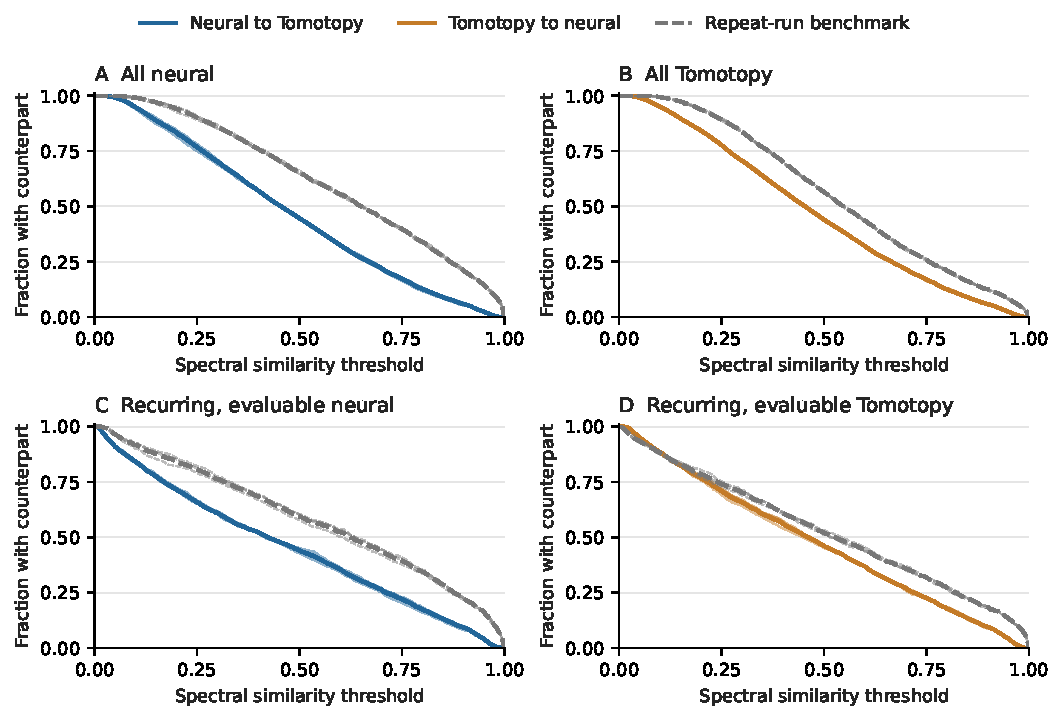
\includegraphics[width=\linewidth]{figures/cross_model_recovery.pdf}
\caption{Bidirectional recovery relative to repeat runs. Colored curves show
neural-to-Tomotopy (blue) or Tomotopy-to-neural (orange) recovery; grey dashed
curves use other fits of the source model. Panels A--B include all 1,000
topics; C--D include recurring, evaluable topics, averaging
\ChemSelectedRecurring{} neural and \ChemLDARecurring{} Tomotopy motifs
per fit. The horizontal axis is the full-$\beta$ similarity required of a
counterpart; the vertical axis is the fraction of the entire source cohort
meeting it. Thin lines are three source-fit summaries, each averaging target
fits, and thick lines are their mean. They are not confidence intervals.
No target fit is pooled with another and no threshold is treated as a
chemical-correctness boundary.}
\label{fig:cross-model-recovery}
\end{figure}

The cohort definition changes the question as well as the number of motifs.
Requiring recurrence without a MAG annotation gives cross-model median-score
summaries of \OverlapNLNoMAGFilterCos{} and \OverlapLNNoMAGFilterCos{},
respectively. Annotation availability therefore affects which patterns enter
the comparison. In particular, an analysis restricted to successful matched
pairs can look more similar than recovery of an entire eligible inventory.
Here weak and unmatched source motifs remain visible in every curve.

\subsubsection{Shared fragments do not imply identical chemistry}

Agreement is much stronger in fragments than neutral losses for the closest
recurring, evaluable cross-model pairs. Mean fit-pair median fragment cosine
is \OverlapNLFragment{} from neural motifs to Tomotopy and
\OverlapLNFragment{} in reverse, whereas the corresponding loss cosines are
\OverlapNLLoss{} and \OverlapLNLoss{}.
Giving the two channel cosines equal weight reduces the median
closest-counterpart score to \OverlapNLChannelCos{} and
\OverlapLNChannelCos{} (Supplementary Figure~\ref{supp-fig:cross-model-agreement}D).
High full-spectrum cosine can therefore reflect shared dominant fragments
without close agreement across both channels. These observations depend on
the selected cohort and matching rule; they do not establish which model's
neutral-loss patterns are chemically more accurate.

The matched chemical evidence is also partial. Compound Jaccard summaries
are \OverlapNLCompound{} and \OverlapLNCompound{}, with signed
chemical-effect cosines of \OverlapNLChemical{} and
\OverlapLNChemical{}. The distributions in
Supplementary Figure~\ref{supp-fig:cross-model-agreement}A--B show that higher spectral scores
often accompany stronger feature agreement, but not uniformly. The two
models can describe related fragment patterns while assigning them to
different small compound groups. Agreement with Tomotopy is therefore
corroboration for a shared pattern, not an independent structural annotation.



\subsubsection{Concrete counterparts and one-to-many neighborhoods}

The fixed example rule illustrates why a recovery curve is more informative
than a single overlap percentage (Figure~\ref{fig:cross-model-examples}).
The neural-to-Tomotopy pair nearest the median best score has cosine
\OverlapMedianCos{}, with \OverlapMedianFragmentShared{} directly shared fragment
and \OverlapMedianLossShared{} shared losses
among its top words at 0.01 Da tolerance. The pair nearest the upper decile
has cosine \OverlapUpperCos{}, but still shares only
\OverlapUpperFragmentShared{} top fragments and \OverlapUpperLossShared{}
top losses. Its dominant fragment aligns closely, while the remaining
spectral description differs. Both are spectral probability patterns, not
experimentally confirmed fragmentation assignments.

Allowing multiple counterparts avoids concealing possible splits or merges,
but does not establish that they are common at high similarity.
The source chosen near the upper decile of second-neighbor scores has
closest scores \OverlapMultipleCos{} and \OverlapMultipleSecondCos{}.
It shares \OverlapMultipleFragmentShared{} and
\OverlapMultipleSecondFragmentShared{} top fragments with the two Tomotopy
candidates, respectively, but \OverlapMultipleLossShared{} top losses with
either. The fraction with multiple counterparts
falls rapidly as the required similarity increases
(Supplementary Figure~\ref{supp-fig:cross-model-agreement}C). Thus the present evidence supports
partial, sometimes one-to-many spectral correspondence rather than a
near-identical chemical inventory. This provides a concrete basis for
comparing the neural model's mixture compactness and inference architecture
with the established MS2LDA workflow, without assuming chemical equivalence.

\begin{figure}[!htbp]
\centering
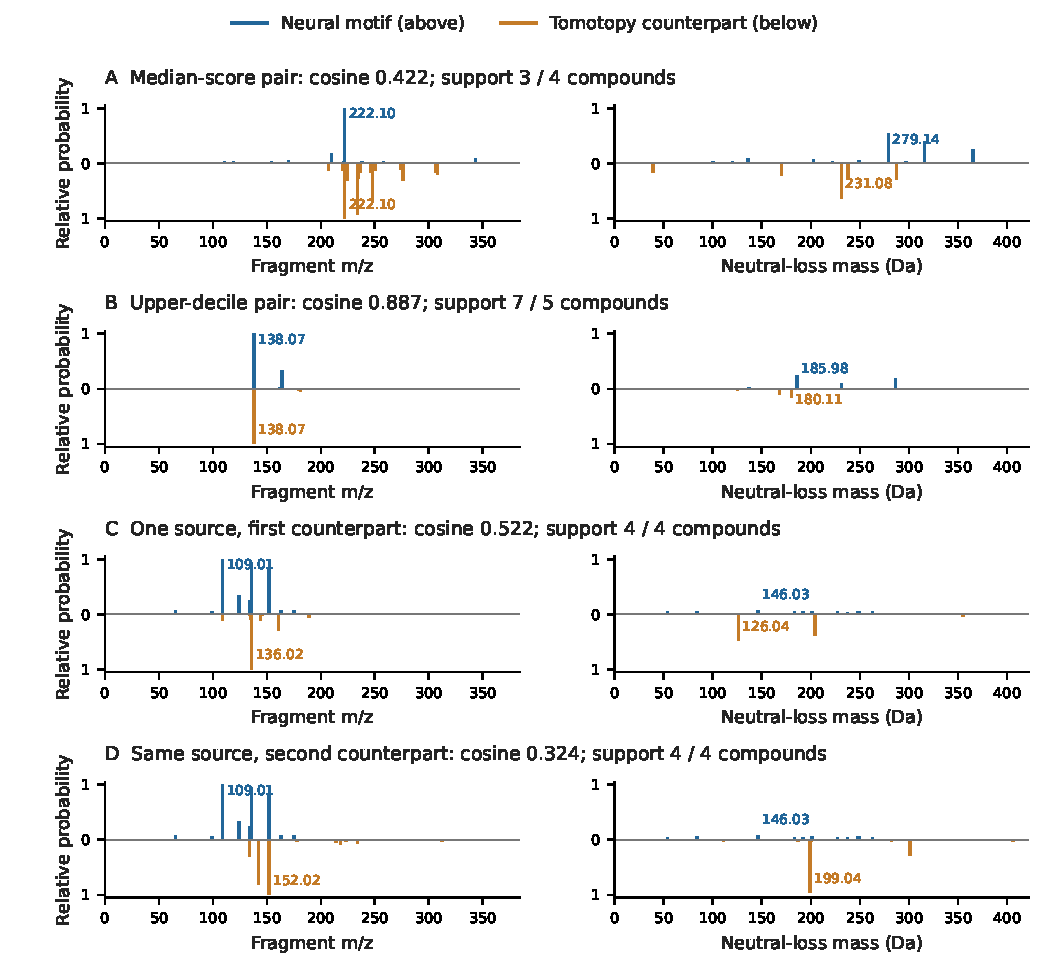
\includegraphics[width=\linewidth]{figures/cross_model_examples.pdf}
\caption{Actual motif counterparts selected by the fixed score-quantile rule.
Neural top-20-word probabilities are plotted above zero and Tomotopy
probabilities below zero, separated into fragment and neutral-loss channels.
Each topic is divided by its own largest word probability across both
channels; these are not measured ion intensities. Axes are shared in mass
range within each column, and labels identify the largest displayed word
in each channel. Support counts are distinct compounds, neural first.
(A) Pair nearest the median closest-counterpart score.
(B) Pair nearest its 90th percentile.
(C--D) The same neural motif and its two nearest Tomotopy counterparts,
chosen near the 90th percentile of second-best scores. The common source
in C--D makes the one-to-many relationship visible without a graph of topic
labels. Exact identities, all probabilities and mass-tolerance sensitivities
are retained in the evidence. Examples are illustrative, not selected for
chemical agreement and not representative chemical validations.}
\label{fig:cross-model-examples}
\end{figure}

\FloatBarrier
\subsection{Chemical specificity beyond common molecular features}
\label{sec:chemical-results}

Both models have a small positive SOS excess over their matched backgrounds,
but the raw overlap is much larger than this excess
(Table~\ref{tab:chemical-assessment}; Figure~\ref{fig:chemical-specificity}A).
The selected model's mean background SOS is \ChemSelectedBackground{},
compared with raw mean SOS \CurrentSOSMean{}; the corresponding Tomotopy
values are \ChemLDABackground{} and \ReferenceLDASOS{}.
Both therefore have mean excess near \ChemSelectedExcess{}.
Details of the matched background are in Supplementary
Section~\ref{supp-sec:background}.
Much of their fingerprint containment can be explained by common features
among compounds with comparable acquisition profiles and precursor masses.
This does not erase the observed associations, but it narrows what a high
raw SOS can establish about chemical specificity.

\begin{table}[H]
\centering\small
\caption{Post-hoc chemical assessment on the fixed MS$^{n}$Lib validation
split. Entries are mean $\pm$ sample SD over three fits per model.
``Evaluable, $\geq2$'' counts MAG-evaluable motifs supported by at least two
distinct compounds. Background SOS is expected overlap among acquisition/mass-matched compounds;
excess SOS is observed minus background overlap. Both are averaged over
evaluable motifs within a fit. ``SOS screen''
counts motifs with conditional SOS $q\leq0.05$; ``Feature screen'' counts
motifs with at least one MACCS key meeting that cutoff, regardless of MAG
availability. Families contain all six fits. Counts are exploratory screens,
not numbers of chemically confirmed discoveries. These descriptive metrics
are not ranked.
Definitions and caveats appear in Section~\ref{sec:chemical-assessment}.}
\label{tab:chemical-assessment}
\setlength{\tabcolsep}{4pt}
\begin{tabular}{@{}lrrrrr@{}}
\toprule
Model & Evaluable, $\geq2$ & Background SOS & Excess SOS & SOS screen & Feature screen \\
\midrule
Tomotopy LDA & $502.7\pm13.0$ & $0.604\pm0.002$ & $0.035\pm0.001$ & $9.7\pm3.5$ & $12.0\pm3.0$ \\
Contextual Sparse ETM & $514.7\pm14.2$ & $0.594\pm0.003$ & $0.035\pm0.003$ & $10.7\pm1.5$ & $10.0\pm1.7$ \\
\bottomrule

\end{tabular}
\end{table}

Support explains an important part of the inventory difference. Among
MAG-evaluable motifs, \ChemSelectedSingletonEligible{} in the selected model
and \ChemLDASingletonEligible{} in Tomotopy are supported by only one
compound, averaged over fits. Requiring at least two compounds reduces the
evaluable inventories to \ChemSelectedRecurring{} and \ChemLDARecurring{},
respectively. The larger neural inventory is therefore not equivalent to
a similarly large increase in recurring, independently supported chemistry.
Figure~\ref{fig:chemical-specificity}B shows the full support distribution,
including supported motifs without a MAG annotation.

\begin{figure}[H]
\centering
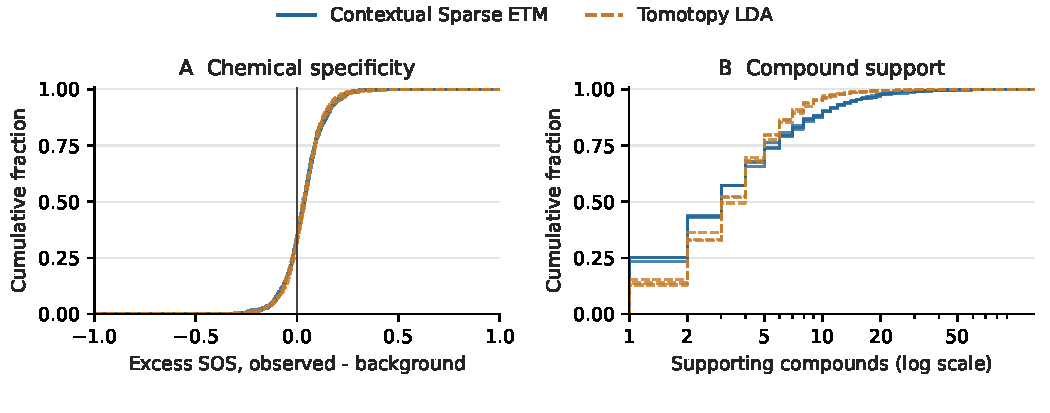
\includegraphics[width=\linewidth]{figures/chemical_specificity.pdf}
\caption{Chemical specificity and compound support, with one curve per fit.
(A) Empirical cumulative distribution of SOS excess over the 50 Da
acquisition-matched background, among evaluable motifs
(\ChemSelectedEligibleMin{}--\ChemSelectedEligibleMax{} per selected fit;
\ChemLDAEligibleMin{}--\ChemLDAEligibleMax{} per Tomotopy fit).
The vertical line denotes no excess.
(B) Cumulative distribution of distinct-compound support among all supported
motifs (\ChemSelectedSupportedMin{}--\ChemSelectedSupportedMax{} selected;
\ChemLDASupportedMin{}--\ChemLDASupportedMax{} Tomotopy), on a logarithmic
count axis.
These curves describe different motif inventories, not paired chemical
identities or independent observations for significance testing.}
\label{fig:chemical-specificity}
\end{figure}

Only a small subset passes the conservative exploratory screens:
\ChemSelectedSOSTopics{} versus \ChemLDASOSTopics{} motifs per fit for SOS,
and \ChemSelectedFeatureTopics{} versus \ChemLDAFeatureTopics{} for at least
one enriched MACCS feature. The latter tests are independent of MAG
availability, not statistically independent of the SOS analysis.
Detected features include bromine presence (key 46) in both models and
sulfur in a ring (key 36) in selected-model motifs. These are interpretable
structural associations, but a key does not specify a fragmentation pathway
or a uniquely identified molecular substructure.

The small positive mean excess persists with alternative mass-bin widths
of 25 and 100 Da (Supplementary Section~\ref{supp-sec:background}). In the scaffold-balanced analysis it is
\ChemSelectedScaffoldExcess{} for the selected model and
\ChemLDAScaffoldExcess{} for Tomotopy. The feature screen then retains only
\ChemSelectedScaffoldFeatureTopics{} and \ChemLDAScaffoldFeatureTopics{}
motifs per fit, respectively. That reduction reflects changed structural
composition and reduced support; it does not by itself distinguish confounding
from loss of power. Together, the analyses support some chemical structure
in both inventories, without establishing a neural advantage in specificity.

\subsection{Spectral repeatability does not imply identical compound groups}

The selected model has higher within-model spectral repeatability than
Tomotopy in these saved fits. The mean of the three pairwise median
full-$\beta$ cosines is \ChemSelectedMatchMedian{} for the selected model
and \ChemLDAMatchMedian{} for Tomotopy (Figure~\ref{fig:motif-correspondence}A).
The mean reciprocal-nearest fraction is \ChemSelectedReciprocal{} versus
\ChemLDAReciprocal{}. Across models, the mean of nine pairwise median
cosines is lower, at \ChemCrossMatchMedian{}: their inventories are not
simply relabelled copies of one another. These descriptive pair summaries
are correlated because they reuse the same fits.
Neural repeats share the same fixed word embeddings, so this repeatability
is conditional on that representation; sensitivity to re-learning the
embeddings is not measured.

The supporting molecules are less repeatable than the spectral patterns.
The mean within-model median compound Jaccard is
\ChemSelectedCompoundMatch{} for the selected model and
\ChemLDACompoundMatch{} for Tomotopy. Different runs can assign similar
spectral motifs to different compounds, particularly when each motif has
few dominant-topic associations. Feature-effect profiles and top-word
overlaps are provided alongside these matches in the supporting evidence;
neither forced matching nor similar spectra establishes identical chemistry.

Within-fit redundancy also cautions against reading motif counts as counts
of distinct substructures. Nearest-topic similarity and repeated MAG
fingerprints are reported in Supplementary Section~\ref{supp-sec:diagnostics}.

\begin{figure}[H]
\centering
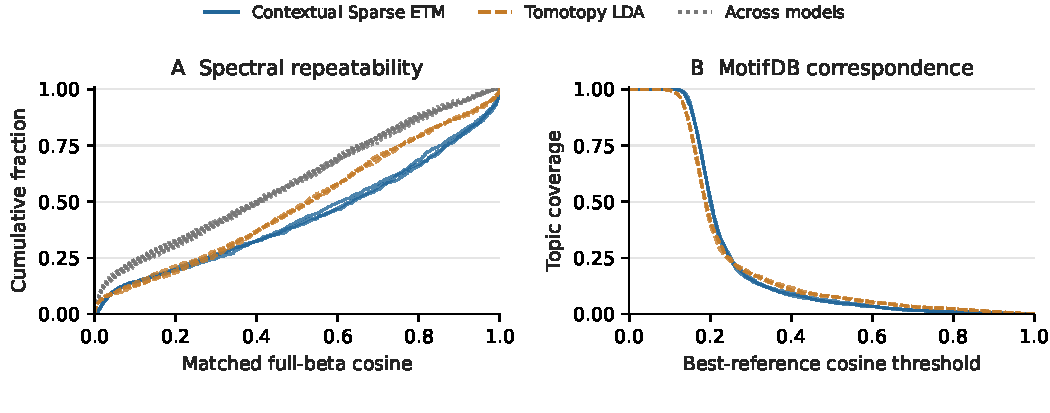
\includegraphics[width=\linewidth]{figures/motif_correspondence.pdf}
\caption{Spectral correspondence across fits and to annotated MotifDB
references. (A) Each curve shows all 1,000 Hungarian-matched topic pairs
for one fit pair: three selected-model pairs, three Tomotopy pairs and
nine cross-model pairs. A curve farther right indicates higher matched
cosines; the matches include weak forced assignments. (B) Fraction of
all 1,000 topics per fit whose best-reference Spec2Vec cosine reaches each
threshold. The two panels use different representations: full topic-word
probabilities in A and embedded top-20-word pseudo-spectra in B. Thresholds
in B are displayed continuously, not interpreted as chemical correctness
probabilities.}
\label{fig:motif-correspondence}
\end{figure}

\subsection{MotifDB provides partial corroboration for selected examples}

The \ChemRawReferences{} reference entries reduce to
\ChemUniqueReferences{} distinct typed spectral signatures, all scorable
with the fixed Spec2Vec model. No reference is excluded as malformed;
\ChemConflictingReferences{} deduplicated signatures retain different
manual-label strings. All learned topics also have scorable embeddings.
Most matches are modest: the mean within-fit median best-reference cosine
is \ChemSelectedReferenceMedian{} for the selected model and
\ChemLDAReferenceMedian{} for Tomotopy. The coverage curves cross
(Figure~\ref{fig:motif-correspondence}B), so the small median difference is
not a uniform neural advantage. At 0.01 Da, the best reference directly
matches an average fraction \ChemSelectedReferenceOverlap{} of the 20
query words for the selected model, compared with
\ChemLDAReferenceOverlap{} for Tomotopy.

\begin{table}[H]
\centering\small
\caption{Illustrative selected-model matches: the three highest-cosine,
distinct reference signatures among recurring motifs with nonzero direct
overlap. These are not a representative sample. Reference labels are
shortened for display, not assigned as confirmed identities of the learned
motifs. ``Compounds'' is distinct motif support; ``Cosine'' is Spec2Vec
similarity. Fragment and loss columns show matched/query feature counts
at 0.01 Da. Examples 2 and 3 match distinct reference signatures carrying
the same structural description. Full fit/topic IDs, labels, source IDs,
reference denominators and tolerance sensitivities are retained in the
generated evidence summary.}
\label{tab:reference-examples}
\setlength{\tabcolsep}{4pt}
\begin{tabularx}{\linewidth}{@{}rXrrrr@{}}
\toprule
Example & Reference description & Compounds & Cosine & Fragments & Losses \\
\midrule
1 & Fragment indicative for aromatic compounds related to methylbenzene substructure & 36 & 0.950 & 1/4 & 0/16 \\
2 & Fragments indicative for dihydroxylated benzene ring substructure & 19 & 0.945 & 2/3 & 0/17 \\
3 & Fragments indicative for dihydroxylated benzene ring substructure & 20 & 0.942 & 2/2 & 0/18 \\
\bottomrule

\end{tabularx}
\end{table}

The strongest examples illustrate both the value and the limits of
reference matching. An aromatic-fragment reference can closely resemble
the dominant part of a motif while explaining only one of its twenty words;
the dihydroxylated-benzene examples share two fragment masses but no losses
(Table~\ref{tab:reference-examples}). High embedding similarity therefore
need not mean complete motif agreement. These matches offer hypotheses
for inspection, not confirmation that each annotated substructure is
present in every supporting molecule. Weak reference correspondence likewise
cannot be used to claim novel chemistry.

\section{Discussion}
\label{sec:discussion}

\subsection{Discovery breadth, chemical specificity and predictive fit}

Our model produces more motifs meeting the usefulness criterion than Tomotopy
on the same validation data (Table~\ref{tab:validation}). The difference in
mean useful-motif count is \CurrentUsefulDifference{}, providing more candidates
for chemical interpretation. Additional motifs need not represent additional
unique substructures, however. Several motifs may describe related chemistry
or different fragmentation behavior of the same substructure, so a larger
number of motifs does not necessarily provide more independent chemical information.

The compound-level assessment sharpens this distinction. Both models show
a small positive SOS excess after accounting for common fingerprint features
within matched acquisition/mass groups, with no clear difference in average
excess. Moreover, much of the larger evaluable neural inventory consists
of motifs supported by a single compound. The gap becomes much smaller
when recurrence across compounds is required. Thus the main evidence favors
broader candidate generation, not a proportional increase in chemically
specific, recurring substructures. The enriched MACCS features and selected
reference matches provide useful starting points for interpretation, but
their restricted support and overlapping descriptions prevent a direct
count of unique chemical discoveries.

The directed comparison with Tomotopy is an important qualification to this
discovery claim. It demonstrates shared spectral patterns, including close
counterparts, while retaining the source motifs that do not match well.
Recurring Tomotopy motifs are partly recovered by the neural model, but
cross-model recovery remains below within-model repeatability. Fragment
agreement is much stronger than neutral-loss agreement, and supporting
compound groups often differ. The result is evidence of partial continuity
with established MS2LDA outputs, not a claim that two implementations discover
the same chemical substructures. Neither agreement nor disagreement alone
decides whether a motif is chemically valid.

Repeatability adds a different consideration. Neural spectral patterns match
more closely across runs, while dominant-topic compound groups remain
unstable in both models. Spectral repeatability is useful for selecting
motifs to inspect, but is not the same as stable assignment of a molecular
class. The repeated MAG profiles and partial reference overlaps further
show that a motif inventory contains overlapping levels of description,
from broad chemical features to more specific fragment patterns.

Predictive fit reveals a further trade-off. Completion NLL is lower
than Tomotopy's but higher than plain ETM's, even though plain ETM produces
far fewer useful motifs. Plain ETM also has slightly higher conditional mean
SOS than the selected model. The preferred model therefore depends on whether
priority is given to word prediction, conditional SOS, or useful-motif count
and compact assignments. Count likelihood and
MAG/SOS measure different properties: spectral-word prediction and
library-dependent structural agreement. They should be assessed separately,
and sparse mixtures alone are not sufficient reason to accept poorer predictions.

\subsection{Compact mixtures and the ETM foundation}

Local sparsity can coexist with broad use of topics across the corpus.
The selected model has a median entropy-effective count of about 3.7 topics
per spectrum, while about 807 topics dominate at least one validation spectrum.
Entmax permits exact zero topic weights, and the fitted model uses many
different topics despite its compact per-spectrum mixtures. The synthetic
experiments show a similar pattern when the planted motifs are known.
However, the gap between word and mixture recovery shows that accurate
relative assignments need not imply equally accurate spectral patterns.
Mixture size and topic counts should therefore be interpreted alongside
recovery and chemical evaluation, rather than judged against a single threshold.

The model builds on the published ETM, retaining its embedding-based
topic--word decoder, Gaussian latent variables, MLP inference network and
latent-space variational objective. The enhancements modify three parts of
this model: balanced channels separate fragment and loss normalization,
contextual evidence shifts the
Gaussian posterior mean using the shared embedding geometry, and entmax
changes the induced topic-mixture distribution. The resulting topics remain
normalized word distributions that can be inspected as spectral motifs.
The MLP is retained from ETM rather than introduced as a new component.

The plain-ETM comparison assesses the combined enhancements rather than
each component separately. Earlier ablations in related model variants
provide more limited evidence for particular mechanisms, as summarized in
Supplementary Section~\ref{supp-app:ablations}; they do not test every combination of enhancements
in the final model. Together, these results support the combined ETM extension
and document its trade-off between motif discovery and predictive fit.
They do not establish that every component is necessary in all settings or
that no simpler model could achieve similar results.

\subsection{Limitations of the current evidence}

We used the same validation data to select the model and report its performance.
Repeated fits describe training variability on those data, but do not remove
selection bias or show how performance varies across new chemical populations.
The reserved test data were also used during earlier development and therefore
cannot provide independent confirmation of the selected model. Three fits
per model do not establish statistical significance. In the plain-ETM comparison,
the original batch size is retained and one fit used a different operating
environment. That comparison does not fully separate architectural effects
from optimization and runtime differences, even with fixed data and matching
scientific package versions.

The observation model introduces further restrictions. Pseudo-counts,
two-decimal bins and a fixed vocabulary make spectra compatible with a topic
likelihood, but fragment and loss words from the same peak are dependent
even though the multinomial treats token draws as conditionally independent.
The pseudo-count scale also fixes the balance between reconstruction and
KL regularization.
Equal channel mass and the sparse Gaussian-derived prior impose additional
assumptions that may not suit every dataset. Similarly, recovery in one
18-motif simulator shows behavior under its construction, rather than validating
real fragmentation mechanisms or robustness across all spectral settings.

Chemical evaluation is constrained by its reference library and association
rule. Connectivity filtering prevents an evaluated molecule from serving as
its own annotation evidence, but cannot remove all related structures or
acquisition biases. Assigning each spectrum to its dominant topic provides
a common comparison rule while excluding secondary motifs from chemical
scoring. The SOS cutoff defines a screening criterion rather than
validating a molecular substructure. The new conditional nulls make that
limitation more explicit, but cannot eliminate residual dependence among
related structures or guarantee exchangeability within strata. Their
multiplicity-adjusted values are exploratory because the model was selected
on these data. Scaffold balancing reduces overrepresentation but also
reduces statistical power. Finally, MotifDB coverage is limited and its
Spec2Vec matching is partly correlated with MAG. These automated checks
can prioritize motifs without expert input; none confirms a fragmentation
mechanism or a novel substructure on its own.

Cross-model matching has its own limits. A closest counterpart is the maximum
over many candidates and can share a dominant peak without the remaining
pattern. Candidate-set sizes, annotation availability and channel weighting
all affect recovery, which is why we retain complete denominators and report
the sensitivities. One-to-many spectral neighbors can reflect overlapping
features rather than a clean chemical subdivision. Moreover, comparison
with Tomotopy does not create an independent reference standard: both models
use the same spectra, vocabulary and downstream annotation resources.

\subsection{Implications for validation and future encoders}

To assess how well these findings generalize, the model should be compared
with Tomotopy on data not used for model development or selection. Such a
comparison should set the evaluation criteria in advance and use comparable
training and inference conditions for both models. The present automated
assessment provides a reproducible way to select motifs for that next study:
consider effect above background, support across compounds and scaffolds,
repeatability, and agreement with concrete reference features together.
The next chemical step is to inspect the supporting spectra and test the
proposed structural relationships, rather than attach a definitive label
from a high embedding score. Independent molecules and, where available,
targeted standards or expert structural assessment would help distinguish
new chemical information from alternative descriptions of shared chemistry.

The partial agreement also clarifies which practical advantages should be
tested next. Tomotopy can infer topics for previously unseen spectra; the
neural distinction is reuse of a learned inference function rather than
iterative document-specific inference. Latency, throughput and memory should
therefore be compared at comparable predictive and motif quality before
claiming a computational advantage. More compact mixtures and greater
spectral repeatability are observed here, but neither automatically implies
faster inference or superior chemical annotation.

The Gaussian inference network also provides a way to incorporate richer
spectral representations. A future encoder could predict Gaussian means and
log variances directly from spectra, or from DreaMS representations, while
retaining the current topic decoder and its interpretation \cite{bushuiev2026}.
Such an extension would require separate evaluation. During document completion,
neither the encoder nor the contextual pathway could use withheld peaks.
Replacing the encoder would not eliminate tokenization from the complete
model: its likelihood and motif representation would still depend on discrete
spectral words. Modeling continuous spectra at the output would require a
separate change to the observation model.

\section{Conclusion}
\label{sec:conclusion}

Contextual Sparse ETM adapts the published Embedded Topic Model through
balanced fragment/loss emissions, whole-spectrum contextual posterior evidence
and 1.5-entmax mixtures. It preserves an explicit topic--word representation
and the neural Gaussian inference backbone while producing compact
per-spectrum assignments alongside broad topic use across the corpus.

Across three training runs evaluated on the MS$^{n}$Lib validation split, the model produces more
motifs meeting the usefulness criterion and lower completion NLL than Tomotopy,
but lower mean chemical overlap among evaluable motifs. Automated chemical
assessment finds modest background-adjusted agreement in both models,
many single-compound candidates, and limited reference corroboration.
Directed recovery identifies shared spectral patterns with Tomotopy but
also substantial unmatched or weakly matched portions of both inventories.
The closest cross-model counterparts agree more strongly in fragments than
neutral losses, so this continuity does not establish chemical equivalence.
The neural model's greater spectral repeatability does not establish stable
compound assignments or more unique substructures. These results support
the model as a candidate-generation method with an inspectable ETM foundation,
while keeping its chemical claims narrower than its motif counts.
Independent evaluation and structural follow-up are needed to determine
which candidates provide reproducible new chemical information.

\section*{Data and code availability}

Public input and annotation assets are distributed in Zenodo record 20179680
\cite{msnlibdata}. Research code, manuscript sources and versioned evidence
are available in the
\href{https://github.com/joewandy/MS2LDA/tree/experiment/minimal-neural-topic-model}{public research branch of the MS2LDA fork}.
The implementation, evidence locations and reproduction
settings are described in Supplementary Section~\ref{supp-app:repro} and the accompanying source
inventory. The neural model remains an isolated research path; the production
MS2LDA Tomotopy backend is unchanged.

% Shared bibliography for the main paper and supplementary information.
\begin{thebibliography}{99}
\bibitem{vanderhooft2016}
J. J. J. van der Hooft, J. Wandy, M. P. Barrett, K. E. V. Burgess, and
S. Rogers. \emph{Topic modeling for untargeted substructure exploration in
metabolomics}. PNAS 113, 13738--13743 (2016).
\url{https://doi.org/10.1073/pnas.1608041113}

\bibitem{torresortega2026}
L. R. Torres Ortega et al. \emph{Large-scale discovery and annotation of
substructure patterns in mass spectrometry profiles}.
Nature Communications 17, 8350 (2026).
\url{https://doi.org/10.1038/s41467-026-75038-0}

\bibitem{blei2003}
D. M. Blei, A. Y. Ng, and M. I. Jordan. \emph{Latent Dirichlet Allocation}.
JMLR 3, 993--1022 (2003).
\url{https://jmlr.org/papers/v3/blei03a.html}

\bibitem{dieng2020}
A. B. Dieng, F. J. R. Ruiz, and D. M. Blei. \emph{Topic Modeling in Embedding
Spaces}. TACL 8, 439--453 (2020).
\url{https://doi.org/10.1162/tacl_a_00325}

\bibitem{srivastava2017}
A. Srivastava and C. Sutton. \emph{Autoencoding Variational Inference for
Topic Models}. ICLR (2017).
\url{https://openreview.net/forum?id=BybtVK9lg}

\bibitem{mikolov2013}
T. Mikolov et al. \emph{Distributed Representations of Words and Phrases
and their Compositionality}. NeurIPS (2013).
\href{https://proceedings.neurips.cc/paper/2013/hash/9aa42b31882ec039965f3c4923ce901b-Abstract.html}{NeurIPS proceedings entry.}

\bibitem{huber2021}
F. Huber et al. \emph{Spec2Vec: Improved mass spectral similarity scoring
through learning of structural relationships}. PLOS Computational Biology 17,
e1008724 (2021).
\url{https://doi.org/10.1371/journal.pcbi.1008724}

\bibitem{peters2019}
B. Peters, V. Niculae, and A. F. T. Martins. \emph{Sparse Sequence-to-Sequence
Models}. ACL, 1504--1519 (2019).
\url{https://doi.org/10.18653/v1/P19-1146}

\bibitem{brungs2025}
C. Brungs et al. \emph{MS$^{n}$Lib: efficient generation of open multi-stage
fragmentation mass spectral libraries}. Nature Methods 22, 2028--2031 (2025).
\url{https://doi.org/10.1038/s41592-025-02813-0}

\bibitem{msnlibdata}
J. Dietrich, J. Wandy, L. R. Torres Ortega, and J. J. J. van der Hooft.
\emph{vdhooftcompmet/MS2LDA: Paper---Data and Models}. Zenodo (2026).
\url{https://doi.org/10.5281/zenodo.20179680}

\bibitem{bemismurcko1996}
G. W. Bemis and M. A. Murcko. \emph{The Properties of Known Drugs. 1.
Molecular Frameworks}. Journal of Medicinal Chemistry 39, 2887--2893 (1996).
\url{https://doi.org/10.1021/jm9602928}

\bibitem{durant2002}
J. L. Durant, B. A. Leland, D. R. Henry, and J. G. Nourse.
\emph{Reoptimization of MDL Keys for Use in Drug Discovery}.
Journal of Chemical Information and Computer Sciences 42, 1273--1280 (2002).
\url{https://doi.org/10.1021/ci010132r}

\bibitem{tomotopy}
M. Lee. \emph{Tomotopy}, release 0.13.0 (2024).
\href{https://github.com/bab2min/tomotopy/releases/tag/v0.13.0}{Official release v0.13.0.}

\bibitem{rogers2019}
S. Rogers, C. W. Ong, J. Wandy, M. Ernst, L. Ridder, and J. J. J. van der Hooft.
\emph{Deciphering complex metabolite mixtures by unsupervised and supervised
substructure discovery and semi-automated annotation from MS/MS spectra}.
Faraday Discussions 218, 284--302 (2019).
\url{https://doi.org/10.1039/C8FD00235E}

\bibitem{panwar2021}
M. Panwar, S. Shailabh, M. Aggarwal, and B. Krishnamurthy.
\emph{TAN-NTM: Topic Attention Networks for Neural Topic Modeling}.
ACL-IJCNLP, 3865--3880 (2021).
\url{https://doi.org/10.18653/v1/2021.acl-long.299}

\bibitem{bushuiev2026}
R. Bushuiev et al. \emph{Self-supervised learning of molecular representations
from millions of tandem mass spectra using DreaMS}.
Nature Biotechnology 44, 630--640 (2026; published online 2025).
\url{https://doi.org/10.1038/s41587-025-02663-3}

\bibitem{pyroprodlda}
Pyro contributors. \emph{Probabilistic Topic Modeling: ProdLDA}.
Official Pyro tutorial, accessed 8 September 2026.
\url{https://pyro.ai/examples/prodlda.html}
\bibitem{phipson2010}
B. Phipson and G. K. Smyth. \emph{Permutation P-values should never be zero:
calculating exact P-values when permutations are randomly drawn}.
Statistical Applications in Genetics and Molecular Biology 9, Article 39 (2010).
\url{https://doi.org/10.2202/1544-6115.1585}

\bibitem{benjamini2001}
Y. Benjamini and D. Yekutieli. \emph{The control of the false discovery rate
in multiple testing under dependency}. Annals of Statistics 29,
1165--1188 (2001).
\url{https://doi.org/10.1214/aos/1013699998}
\end{thebibliography}

\end{document}
